% Light!
\documentclass[8pt, a4paper, oneside, twocolumn]{extarticle}
\usepackage{verbatim}  % for multiline comments
\begin{comment}
The options oneside and twoside affect the width of the side margins.  With oneside , which is the default for article, report, and letter, the margins on both  sides  of  every  page  are  equally  wide.   With twoside, Latex distinguishes between an inner and outer  margin.   The  outer  margin  is  substantially wider  and  switches  between  left  and  right.   Even pages have their outer margin on the left, odd pages on the right.  Most books follow this structure and so it should not come as a surprise that the book class default is twoside.
The standard Latex classes (article, report etc) support ten, eleven and twelve point text. These are the commonest sizes used in publishing.
However, for certain applications there may be a need for other sizes.
The extsizes classes (extarticle, extreport, extbook, extletter, and
extproc) provide support for sizes eight, nine, ten, eleven, twelve,
fourteen, seventeen and twenty points.	
Also as we want whole document to have two columns, we gave it as an optimal parameter however if we want a particular page to have two columns, the command \twocolumn starts a new page having two columns. Accordingly, \onecolumn starts a new page with a single column assuming you are in a two column environment as described above. Both commans do not take any arguments. 
The is a way to define the distance between the two columns, use
\setlength{\columnsep}{distance}

If you need a line to separate the columns, the following command will do the job:
\setlength{\columnseprule}{thickness}
\end{comment}
\usepackage{graphicx}
\usepackage[export]{adjustbox}
\usepackage[compact]{titlesec}  % documentation: http://mirror.iopb.res.in/tex-archive/macros/latex/contrib/titlesec/titlesec.pdf  
\usepackage{kotex}
\usepackage[left=0.8cm, right=0.8cm, top=2cm, bottom=0.3cm, a4paper]{geometry}
\usepackage{amsmath}
\usepackage{ulem}
\usepackage{amssymb}
\usepackage{minted}  % syntax highlighting
\usepackage{enumitem}
\setlist{nolistsep}
\usepackage{fancyhdr} % documentation: http://ctan.math.utah.edu/ctan/tex-archive/macros/latex/contrib/fancyhdr/fancyhdr.pdf
\begin{comment}
The pack­age pro­vides ex­ten­sive fa­cil­i­ties, both for con­struct­ing head­ers and foot­ers, and for con­trol­ling their use (for ex­am­ple, at times when LaTeX would au­to­mat­i­cally change the head­ing style in use).
\end{comment}
\usepackage{lastpage}  % just so that we can use \pageref {LastPage}
\usepackage{color, hyperref}
% The lines in the table of contents become links to the corresponding pages in the document by simply adding in the preamble of the document the line
\begin{comment}
\titlespacing{command}{left spacing}{before spacing}{after spacing}[right]
% spacing: how to read {12pt plus 4pt minus 2pt}
%           12pt is what we would like the spacing to be
%           plus 4pt means that TeX can stretch it by at most 4pt
%           minus 2pt means that TeX can shrink it by at most 2pt
%       This is one example of the concept of, 'glue', in TeX
\end{comment}
\usepackage{tikz}
\newcommand{\swastik}[1]{%
    \begin{tikzpicture}[#1]
        \draw (-1,1)  -- (-1,0) -- (1,0) -- (1,-1);
        \draw (-1,-1) -- (0,-1) -- (0,1) -- (1,1);
    \end{tikzpicture}%
}
\newcommand{\revised}{Should be \textcolor{red}{\textbf{revised}}.}
\newcommand{\tested}{Should be \textcolor{red}{\textbf{tested}}.}
\newcommand{\added}{Should be \textcolor{red}{\textbf{added}}.}
\titlespacing*{\section}
{0pt}{0px plus 1px minus 0px}{-2px plus 0px minus 0px}
\titlespacing*{\subsection}
{0pt}{0px plus 1px minus 0px}{0px plus 3px minus 3px}
\titlespacing*{\subsubsection}
{0pt}{-5px plus 1px minus 0px}{0px plus 3px minus 3px}

\setlength{\columnseprule}{0.4pt}
\pagenumbering{arabic}
\begin{comment}
The  page  headers  and  footers  in  Latex are  defined  by  the 	\pagestyle and \pagenumbering commands. \pagestyle defines the general contents of the headers and footers (e.g.  where the page  number  will  be  printed),  while \pagenumbering defines  the  format  of  the  page  number. Latexhas four standard pagestyles:
empty - no headers or footers
plain - no header, footer contains page number centered
headings - no footer,  header contains name of chapter/section and/or sub-section and page number
myheadings - no footer, header contains page number and user supplied information
The \pagestyle command changes the style from the current page on throughout the remainder of your document.
\end {comment}
\pagestyle{fancy}  % using fancyhdr
\lhead{}
\rhead{Page \thepage  \ of \pageref{LastPage} }
\fancyfoot{}

\headsep 0.2cm  % seperation between header and body
% Automatically break long lines in minted environments and \mint commands, and wrap longer lines in \mintinline.
% the number of tabs is equivalent to
% The symbol used at the beginning (left) of continuation lines when breaklines=true. To have no symbol, simply set breaksymbolleft to an empty string
\setminted{breaklines=true, tabsize=2, breaksymbolleft=}
\usemintedstyle{perldoc} % takes an optional argument to specify the style for a particular language, and works anywhere in the document
\begin {comment}
You can change the values of the variables defining the page layout with two commands. With this one you can set a new value for an existing length variable:

\setlength{\mylength}{length}

with this other one, you can add a value to the existing one:

\addtolength{\mylength}{length}

\itemsep = vertical space added after each item in the list.
\parsep = vertical space added after each paragraph in the list.
\topsep = vertical space added above and below the list.
\partopsep = vertical space added above and below the list, but only if the list starts a new paragraph.

\end{comment}
\begin{document}
\title{\swastik {scale = 0.2} {}Short Revision Notes{} \swastik {scale = 0.2}}
\author{Sourabh Aggarwal (\href {https://codeforces.com/profile/sourabh23}{sourabh23})}
\date{Compiled on \today}
\maketitle
\pagenumbering {roman}
\tableofcontents
\newpage
\thispagestyle{fancy}  % else it was not giving fancy header to the first page
\pagenumbering{arabic}
\noindent\textcolor{red}{\textbf{Think twice code once!}}

\section{Maths}
\subsection{Game Theory}
Games like chess or checkers are partizan type.\\
\subsubsection{What is a Combinatorial Game?}
\begin{enumerate}
\item There are 2 players.
\item There is a set of possible positions of Game
\item If both players have same options of moving from each position, the game is called impartial; otherwise partizan
\item The players move alternating.
\item The game ends when a postion is reached from which no moves are possible for the player whose turn it is to move. Under \textbf {normal play rule}, the last player to move wins. Under \textbf {misere play rule} the last player to move loses.
\item The game ends in a finite number of moves no matter how it is played.
\end{enumerate}
\textbf{P} - Previous Player, \textbf{N} - Next Player
\begin{enumerate}
\item Label every terminal position as P - postion
\item Position which can move to a P position is N position
\item Position whole all moves are to N positoin is P position.
\end{enumerate}
\textbf{Note: } Every Position is either a P or N. \\
Directed graph G = ($X, F$), where $X$ is positions (vertices) and $F$ is a function that gives for each $x \in X$ a subset of $X$, i.e. \textit {followers of $x$}. If $F (x)$ is empty, $x$ is called a terminal position.\\
$g(x) = min \{ n \geq 0 : n \neq g (y)$ for $y \in F (x)\}$\\
Positions $x$ for which $g(x)$ is 0 are P postions and all others are N positions.\\
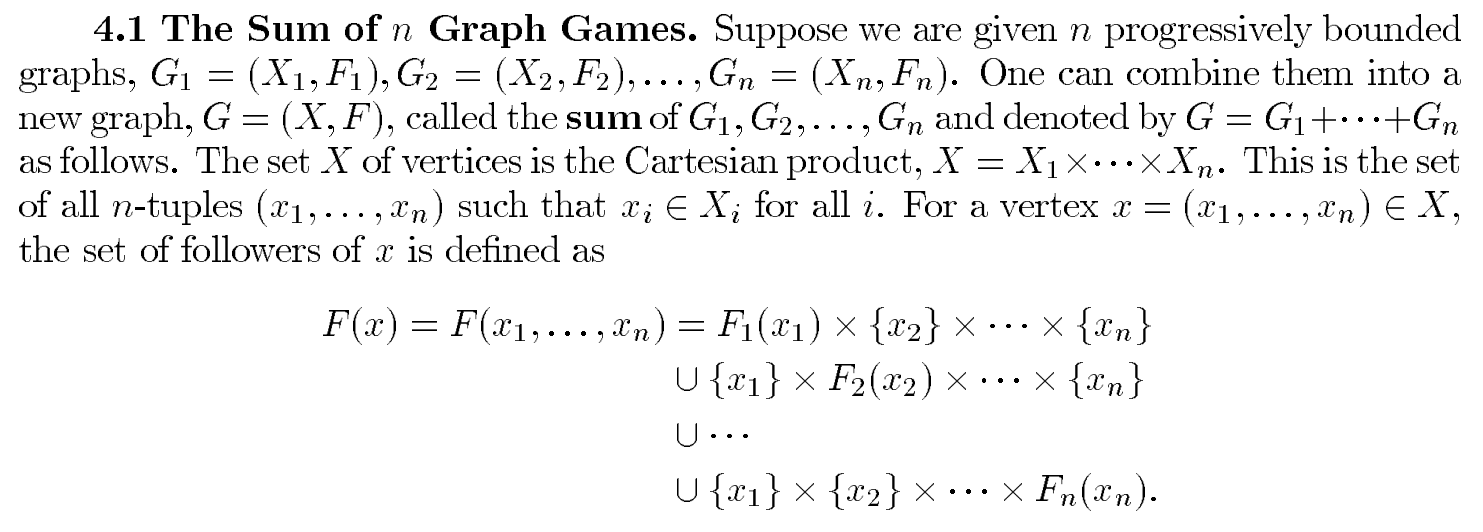
\includegraphics[width=0.5\textwidth,height=0.5\textheight,keepaspectratio]{sumgraph}
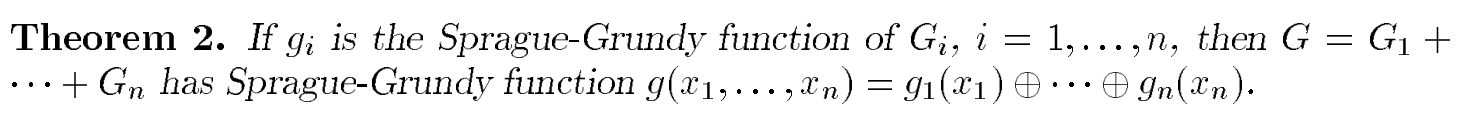
\includegraphics[width=0.5\textwidth,height=0.5\textheight,keepaspectratio]{sgth}
\textbf{Thus}, if a position is a \textbf{N} position, we can cleverly see which position should we go to (which component game move to take) such that we reach \textbf {P} position.
\section{Graphs}
\subsection{Tree}
Undirected, acyclic, connected, $|V| - 1$ edges.\\
All edges are bridges, and internal vertices (degree $> 1$) are articulation points.\\
It is as well a bipartite graph.\\
\textbf{SSSP}: Simply take the sum of edge weights of that unique path. $O(|V|)$\\
\textbf{APSP}: Simply do SSSP from all vertices. $O(|V^2|)$
\begin{minted}{cpp}
void preorder (v) {
	visit (v);
	preorder (left (v));
	preorder (right (v));
}
void inorder (v) {
	inorder (left (v));
	visit (v);
	inorder (right (v));
}
void postorder (v) {
	postorder (left (v));
	postorder (right (v));
	visit (v);
}
\end{minted}
It is \textbf {impossible} to construct binary tree with just Preorder traversal.\\ 
It is \textbf {impossible} to construct binary tree with just Inorder traversal.\\
It is \textbf {impossible} to construct binary tree with just Postorder traversal.
\subsubsection{Important Problems}
\begin{itemize}
	\item \href {https://gist.github.com/sourabh2311/6cff69fef833097556696bd6f31f3f1d}{UVA 11695 Sol}: Problem Desc: Find which edge to remove and add so as to minimise the number of hops to travel between flights.\\
	Problem Sol: Just link the center of diameters. Brute force which edge to remove. 
	\item \href {https://github.com/sourabh2311/Competitive-Programming/blob/master/UVA_112.cpp}{UVA 112 Sol}, \href {https://uva.onlinejudge.org/external/1/112.pdf}{UVA 112 Prob}: Just see how I processed the input.	
	\item \href {https://gist.github.com/sourabh2311/6b761c14bef4e5887e6b03b809bc4983}{UVA 10029 Sol}, \href {https://uva.onlinejudge.org/external/100/10029.pdf}{UVA 10029 Prob}: Edit steps, (lexicographic sequence of words)	
	\item \href {https://gist.github.com/sourabh2311/d73572fab5cf6d390f509d29abf4cd60}{UVA 536 Sol}, \href {https://uva.onlinejudge.org/external/5/536.pdf}{UVA 536 Prob}: Construct binary tree with preorder and inorder	
	\item \href {https://gist.github.com/sourabh2311/25edb7a7067948832ade9192bd2635ce}{UVA 10459 Sol}, \href {https://uva.onlinejudge.org/external/104/10459.pdf}{UVA 10029 Prob}: Edit steps, (lexicographic sequence of words)	
\end{itemize}
\section{Some Basic}
\begin{minted}{cpp}
	while (first || cin >> temp) {  // something }
\end{minted}
\section{Strings}
To map keyboard etc, it is better to create 2 strings then loop through and map.\\
To transform complete string to lowercase: 
\begin{minted}{cpp} 
transform (word.begin (), word.end (), word.begin (), ::tolower); 
\end{minted}
To concatenate two vectors: 
\begin{minted}{cpp}
vector1.insert (vector1.end (), vector2.begin (), vector2.end ()); 
\end{minted}
\begin{minted}{cpp} 
string.substr (startposn, length); // Where startposn is 0 indexed.
\end{minted}
\begin{minted}{cpp}
int pos1 = line.find ("U=");
if (pos1 != -1) { // process }  
line.replace (pos, len, newString); // pos = line.find (f), len = f.size ()
\end{minted}
We can iterate through all substrings of string $O(n^2)$ and see which all of them are palindromes in $O(n^3)$ or in $O(n^2)$ by using dp ($dp[startpos][endpos] = (s[startpos] == s[endpos] \&\& dp[startpos + 1][endpos - 1]$) or hash.
\subsection{Minimum Edit Distance}
\begin{minted}{cpp}
void fillmem() {
   for (int j = 0; j <= a.size(); j++) mem[0][j] = j;
   for (int i = 0; i <= b.size(); i++) mem[i][0] = i;
   for (int i = 1; i <= b.size(); i++) {
       for (int j = 1; j <= a.size(); j++) {
           if (a[j - 1] == b[i - 1]) mem[i][j] = mem[i - 1][j - 1];
           else mem[i][j] = min(mem[i - 1][j - 1], min(mem[i - 1][j], mem[i][j - 1])) + 1;
       }
   }
    // mem[b.size ()][a.size ()] contains the answer
}
void print() {
   int i = b.size(), j = a.size();
   while (i || j) {
       if (i and j and a[j - 1] == b[i - 1]) { i--; j--; continue; }
       if (i and j and mem[i][j] == mem[i - 1][j - 1] + 1) {
           cout << "C" << b[i - 1]; if (j <= 9) cout << "0";
           cout << j;
           i--; j--;
           continue;
       }
       if (i and mem[i][j] == mem[i - 1][j] + 1) {
           cout << "I" << b[i - 1];
           if (j <= 9) cout << "0";
           cout << j + 1;
           i--;
           continue;
       }
       else if (j) {
           cout << "D" << a[j - 1];
           if (j <= 9) cout << "0";
           cout << j;
           j--;
       }
   }
   cout << "E\n";
}
\end{minted}
\subsection{Length of longest Palindrome possible by removing 0 or more characters}
\begin{minted}{cpp}
dp[startpos][endpos] = s[startpos] == s[endpos] ? 2 + dp[startpos + 1][endpos - 1] : max (dp[startpos + 1][endpos], dp[startpos][endpos - 1])
\end{minted}
\subsection{Longest Common Subsequence}
\begin{minted}{cpp}
memset (mem, 0, sizeof (mem));
for (int i = 1; i <= b.size (); i++) {
	for (int j = 1; j <= a.size (); j++) {
		if (b[i - 1] == a[j - 1]) mem[i][j] = mem[i - 1][j - 1] + 1;
		else mem[i][j] = max (mem[i - 1][j], mem[i][j - 1])
	}
}
void printsol (int ui, int li) {
	ui--; li--;
	vector<string> ans;
	while (ui || li) {
		if (a[ui] == b[li]) {
			ans.push_back (a[ui]);
			ui--; li--;
			continue;
		}
		if (ui and mem[ui][li] == mem[ui - 1][li]) {
			ui--;
			continue;
		}
		if (li and mem[ui][li] == mem[ui][li - 1]) {
			li--;
			continue;
		}
	}
	reverse (ans.begin (), ans.end ());
	cout << ans << "\n";
}
\end{minted}
\subsection{Prefix Function and KMP}
\subsubsection{Prefix Function}
The prefix function for this string is defined as an array $\pi$ of length n, where $\pi[i]$ is the length of the longest proper prefix of the substring $s[0 … i]$ which is also a suffix of this substring. A proper prefix of a string is a prefix that is not equal to the string itself. By definition, $\pi[0]=0$. Example:\\
$abcabchejfabcabca$\\
$00012300001234564$\\
\textbf{Note: } $\pi[i + 1] \leq \pi[i] + 1$ as if $\pi[i + 1] > \pi[i] + 1$ then consider this suffix ending at position i + 1 \& having length $\pi[i + 1]$ - removing the last character we get a suffix ending in position i \& having length $\pi[i + 1] - 1$ that is better than $\pi[i]$. Should be able to reason the following code.
\begin{minted}{cpp}
vector<int> prefix_function(string &s) {  // O(n)
    int n = (int)s.length();
    vector<int> pi(n, 0);
    for (int i = 1; i < n; i++) {
        int j = pi[i-1];
        while (j > 0 && s[i] != s[j])
            j = pi[j-1];
        if (s[i] == s[j])
            j++;
        pi[i] = j;
    }
    return pi;
}
\end{minted}
\subsubsection{KMP}
Given a text t and a string s, we want to find and display the positions of all occurrences of the string s in the text t.
\\For convenience we denote with n the length of the string s and with m the length of the text t.\\
We generate the string s+\#+t, where \# is a separator that doesn't appear in s and t. Let us calculate the prefix function for this string. Now think about the meaning of the values of the prefix function, except for the first n+1 entries (which belong to the string s and the separator). By definition the value π[i] shows the longest length of a substring ending in position i that coincides with the prefix. But in our case this is nothing more than the largest block that coincides with s and ends at position i. This length cannot be bigger than n due to the separator. But if equality π[i]=n is achieved, then it means that the string s appears completely in at this position, i.e. it ends at position i. Just do not forget that the positions are indexed in the string s+\#+t.\\
Thus if at some position i we have π[i]=n, then at the position $i − (n + 1) − n + 1 = i − 2n$ in the string t the string s appears.\\
As already mentioned in the description of the prefix function computation, if we know that the prefix values never exceed a certain value, then we do not need to store the entire string and the entire function, but only its beginning. In our case this means that we only need to store the string s+\# and the values of the prefix function for it. We can read one character at a time of the string t and calculate the current value of the prefix function.
\begin{minted}{cpp}
void kmp() {
    auto pref = prefix_function(p);
    int j = 0;
    int cnt = 0;
	// Note: pi[n] = 0, hence j = 0.
    for (int i = 0; i < t.size(); i++) {
        while (j > 0 and t[i] != p[j]) {
            j = pref[j - 1];
        }
        if (t[i] == p[j]) j++;
        if (j == p.size()) {  // j == n, that means we must dec. j. 
		// And remember that if s[0...n - 1] == s[1...n - 1]s[n-1] that means s[0] = s[1], s[1] = s[2], s[n-2] = s[n-1]. That means all characters are same and hence we haven't lost anything as pref[n - 1] = n - 1.
            cnt++;  // occurence found
            j = pref[j - 1];
        }
    }
}
\end{minted}
\subsubsection{Counting number of occurrences of each prefix}
\begin{minted}{cpp}
vector<int> ans(n + 1);
for (int i = 0; i < n; i++)  // Longest prefix is favored and will have correct count. But remember that longest prefix also have smaller prefix in it. So here i is string index
    ans[pi[i]]++;
for (int i = n-1; i > 0; i--)  // here i is prefix length. Thus we are doing backward propagation
    ans[pi[i-1]] += ans[i];
for (int i = 0; i <= n; i++)  // as only intermediate strings were considered, we didn't consider original prefix.
    ans[i]++;
\end{minted}
\subsection{Notes}
\begin{itemize}
    \item In case of hashing a string, we follow polynomial rolling hash function, with p as a prime number roughly equal to the size of character domain and m as a huge prime number.
\end{itemize}
\subsection{SAM}
A suffix automaton for a given string s is a minimal DFA that accepts all the suffixes of the string s.
\begin{itemize}
	\item A suffix automaton is an oriented acyclic graph.
	\item One of the states $t_0$ is the initial state
	\item All transitions originating from a state must have different labels
	\item One or multiple states are marked as terminal states. If we start from the initial state $t_0$ and move along transitions to a terminal state, then the labels of the passed transitions must spell one of the suffixes of the string s. Each of the suffixes of s must be spellable using a path from $t_0$ to a terminal state.
\end{itemize}
Consider any non-empty substring t of the string s. We will denote with endpos(t) the set of all positions in the string s, in which the occurrences of t end. For instance, we have endpos("bc")= \{2,4\} for the string "abcbc".\\
We will call two substrings t1 and t2 endpos-equivalent, if their ending sets coincide i.e. endpos(t1) = endpos(t2). Thus all non-empty substrings of the string s can be decomposed into several equivalence classes according to their sets endpos.\\
It turns out, that in a suffix machine endpos-equivalent substrings correspond to the same state. In other words the number of states in a suffix automaton is equal to the number of equivalence classes among all substrings, plus the initial state.\\
Lemma 1: Two non-empty substrings u and w (with length(u) ≤ length(w)) are endpos-equivalent, if and only if the string u occurs in s only in the form of a suffix of w. (Proof is obvious)\\
Lemma 2: Consider two non-empty substrings u and w (with length(u) ≤ length(w)). Then their sets endpos either don't intersect at all, or endpos(w) is a subset of endpos(u). And it depends on if u is a suffix of w or not. (Proof is obvious)\\
Lemma 3: Consider an endpos-equivalence class. Sort all the substrings in this class by non-increasing length. Then in the resulting sequence each substring will be one shorter than the previous one, and at the same time will be a suffix of the previous one. In other words the substrings in the same equivalence class are actually each others suffixes, and take all possible lengths in a certain interval [x;y].\\
Consider some state v ≠ $t_0$ in the automaton. As we know, the state v corresponds to the class of strings with the same endpos values. And if we denote by w the longest of these strings, then all the other strings are suffixes of w. \textbf{suffix link} \textit{link(v)} leads to the state that corresponds to the longest suffix of w that is another endpos-equivalent class.\\
Lemma 4: Suffix links form a tree with the root $t_0$.\\
Lemma 5: If we build a endpos tree from all the existing sets (according to the principle “the set-parent contains as subsets of all its children”), then it will coincide in structure with the tree of suffix references.\\
Note: For each state v one or multiple substrings match. We denote by longest(v) the longest such string, and through len(v) its length. We denote by shortest(v) the shortest such substring, and its length with minlen(v). Then all the strings corresponding to this state are different suffixes of the string longest(v) and have all possible lengths in the interval [minlength(v);len(v)]. For each state v ≠ $t_0$ a suffix link is defined as a link, that leads to a state that corresponds to the suffix of the string longest(v) of length minlen(v)$ − 1$. minlen(v) = len(link(v))+1 \\
Number of states in suffix automaton of the string s of length n doesn't exceed $2n - 1$ (for n $\geq$ 2)\\
Number of transitions $\leq 3n - 4$.
\subsection{Important Problems}
\textit{Review: cf 631D}
\begin{itemize}
	\item \href {https://github.com/sourabh2311/Competitive-Programming/blob/master/UVA_10739.cpp}{UVA 10739 Sol}, \href {https://uva.onlinejudge.org/external/107/10739.pdf}{UVA 10739 Prob}: String to palindrom, just see the minimum edit distance between this string and its reverse but need to divide by 2 later as both strings are it itself.	
	\item \href {https://codeforces.com/contest/245/problem/H}{Queries for the number of palindromic substrings within given range}, \href {https://github.com/sourabh2311/Competitive-Programming/blob/master/IMP%20QUES/Suffix%20String%20Structure/Hash/514C%20-%20Watto%20And%20Mechanism.cpp}{\textbf {See this soln to see power of hashing.}}: 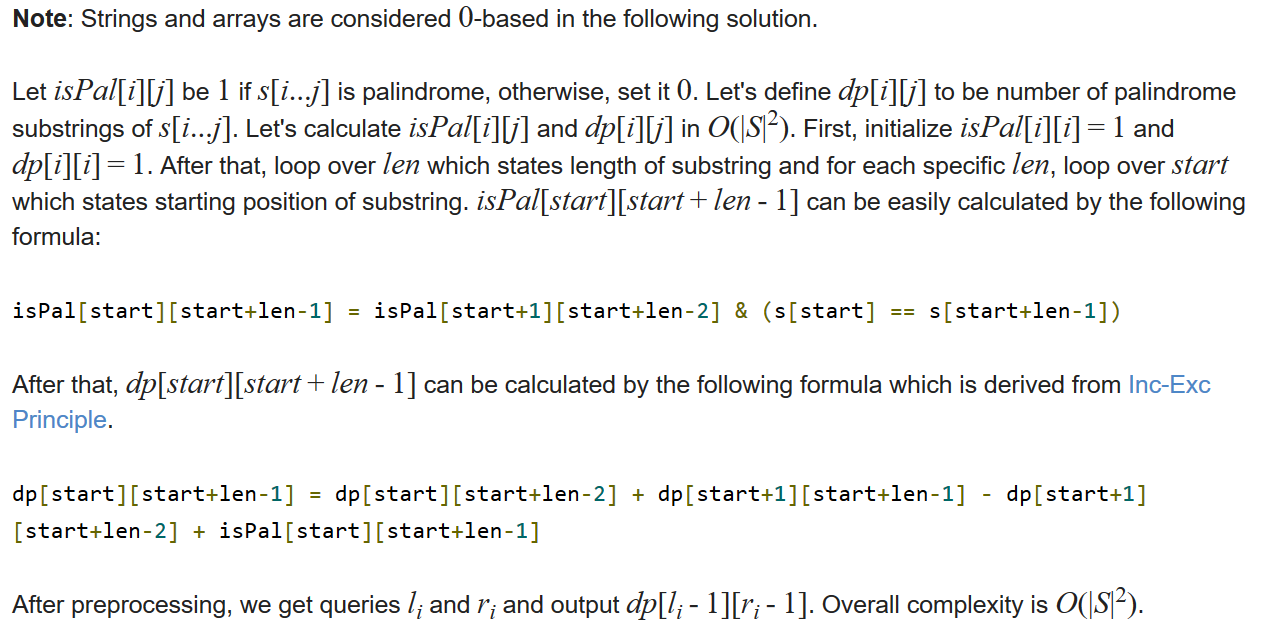
\includegraphics[width=0.5\textwidth,height=0.5\textheight,keepaspectratio]{palsub} 	
	\item \href {https://gist.github.com/sourabh2311/d73572fab5cf6d390f509d29abf4cd60}{UVA 536 Sol}, \href {https://uva.onlinejudge.org/external/5/536.pdf}{UVA 536 Prob}: Construct binary tree with preorder and inorder	
	\item \href {https://gist.github.com/sourabh2311/25edb7a7067948832ade9192bd2635ce}{UVA 10459 Sol}, \href {https://uva.onlinejudge.org/external/104/10459.pdf}{UVA 10029 Prob}: Edit steps, (lexicographic sequence of words)	
\end{itemize}
\end{document}
